\documentclass[9pt,pdftex]{beamer}

% use git: import repository as new project in eclipse: http://www.eclipse.org/forums/index.php/t/226301/

\usepackage[utf8]{inputenc}
\usepackage[english]{babel}
\usepackage{amsfonts, amsmath, amssymb}
\usepackage{color}
\usepackage{fancybox}
\usepackage{graphicx}
\usepackage{multirow}
% \usepackage{paralist}
\usepackage{todonotes}
%\usepackage{biblatex}
\usepackage{subfig}
\newenvironment{figure*}%
{\begin{figure}}
{\end{figure}}

%\usepackage[style=mla,babel=hyphen,backend=biber]{biblatex}

% CSE-Beamer-Styles:
%\usepackage[conference]{beamertheme_sccstalk}
\usepackage[lecture]{beamertheme_sccstalk}
\usepackage{beamercolorscheme_sccs}
\usepackage{beamerfontthemestructurebold}

\graphicspath{{img/}}

\setcounter{tocdepth}{3} 

\title{Simulation of the air flow in the MI building with LBM}
\subtitle{CFD Lab Project: midterm presentation}
\author[Group 02]{Group 02: Martin Andreev, Gerasimos Chourdakis, Igor Tominec} %[displayed in footer]{displayed on title page}
\date{\today}
\institute{Technische Universität München}

\begin{document}
	\frame{\titlepage}

	%===========================================================================
\section*{Contents}
\begin{frame}{Contents}
\tableofcontents
\end{frame}
	
%===========================================================================

\section{The idea}

\begin{frame}{}
\begin{figure}
 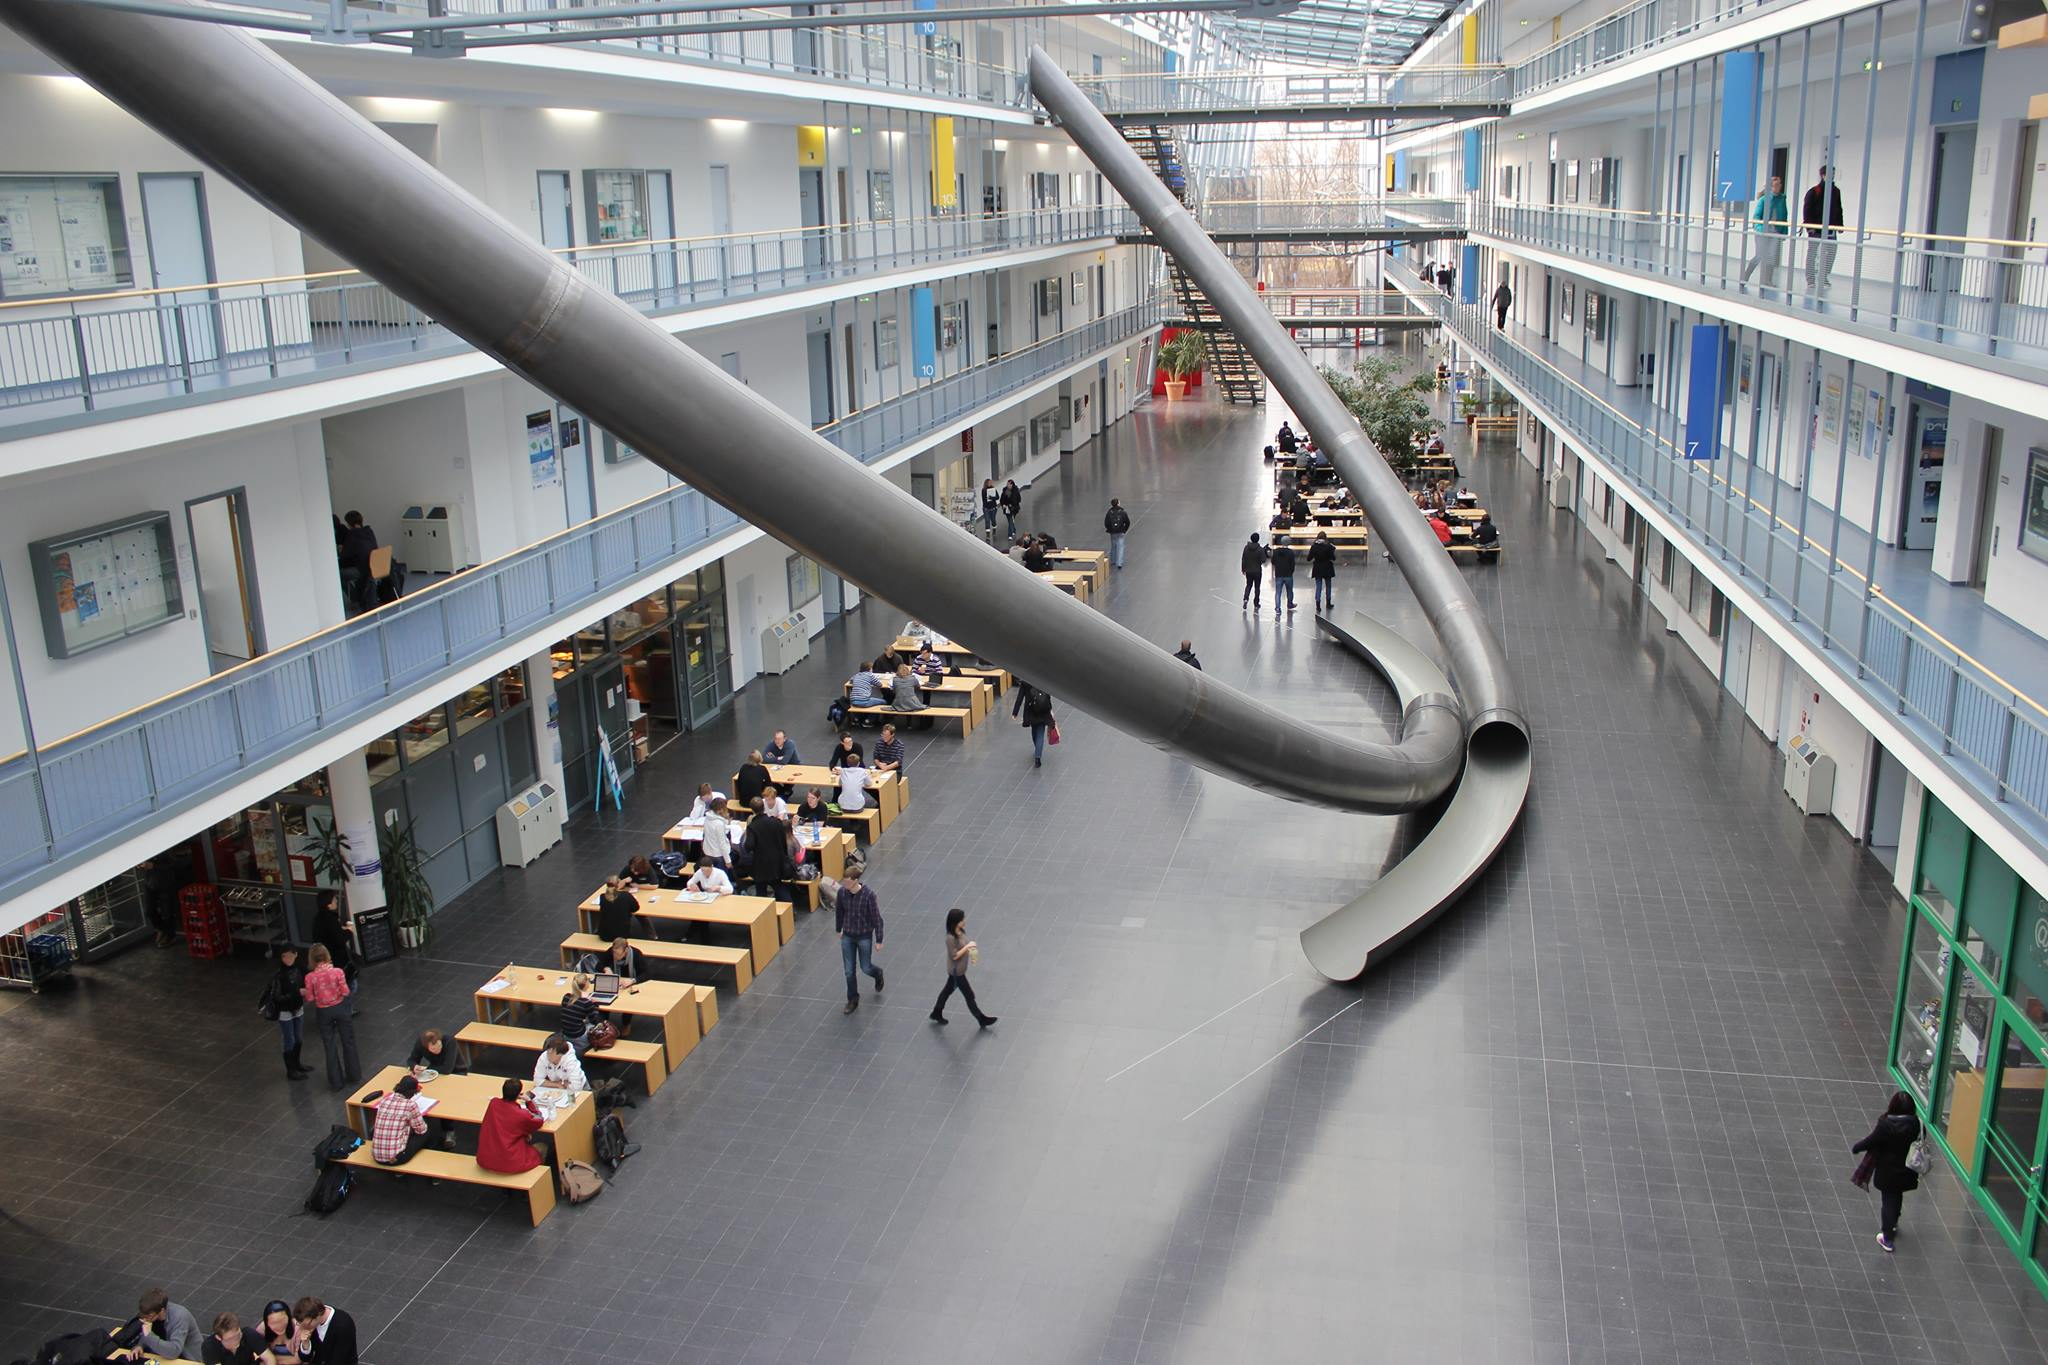
\includegraphics[scale=0.13]{MI_slides}
\end{figure}
\end{frame}

\subsection{What we want to do}
\begin{frame}{What we want to do}
 We want to simulate the airflow in a complex geometry with LBM. 
 
 Why not our building?!
 
 It may be quite a big scale but... let's try it!

\end{frame}

\subsection{What we need}
\begin{frame}{What we need}
 We need:
 \begin{itemize}
  \item The geometry of the building
  \item Boundary conditions (types, parameters)
  \item Flow parameters (viscosity, Reynolds)
  \pause
  \item We need all these dimensionless!
  \pause
  \item And we also need a fine grid...
 \end{itemize}
\end{frame}

\begin{frame}{What we need (2)}
 Because we need a fine grid, we will need a parallel approach.
 
 So we also need:
 \begin{itemize}
  \item To \textbf{merge} our parallel and our arbitrary-geometries code
  \item To invent a way of \textbf{separating the complex domain}
  \item To \textbf{balance the work} among different processors
  \item To effectively \textbf{transfer information} between different subdomains
 \end{itemize}
\end{frame}

\section{Geometry approach}
\begin{frame}{How to extract the geometry?}
 \begin{figure}
 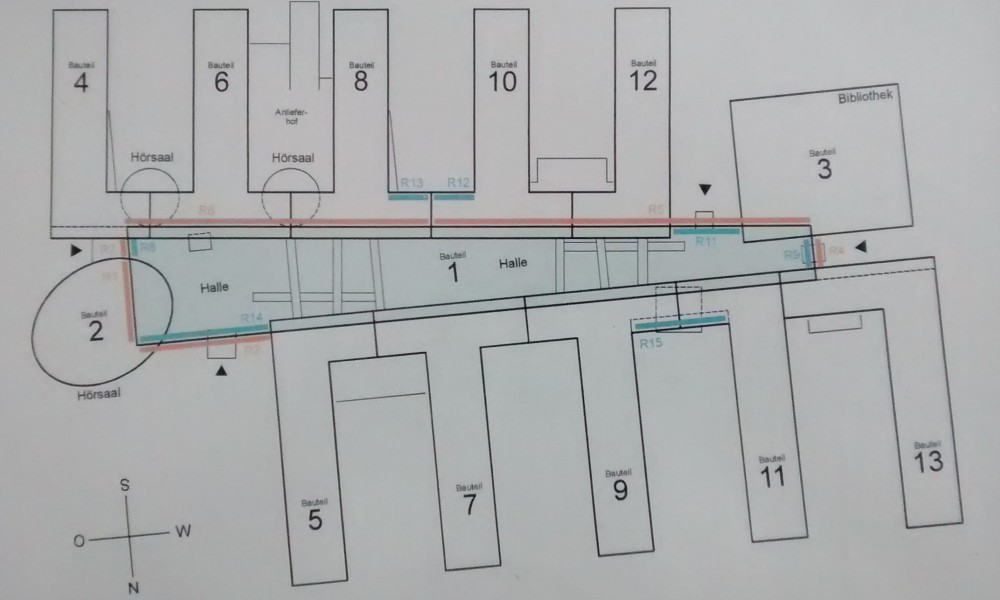
\includegraphics[scale=0.25]{fire_plan}
\end{figure}
\pause Well, we are assuming some simplifications...
\end{frame}

\begin{frame}{How to know the sizes?}
  \begin{figure}
 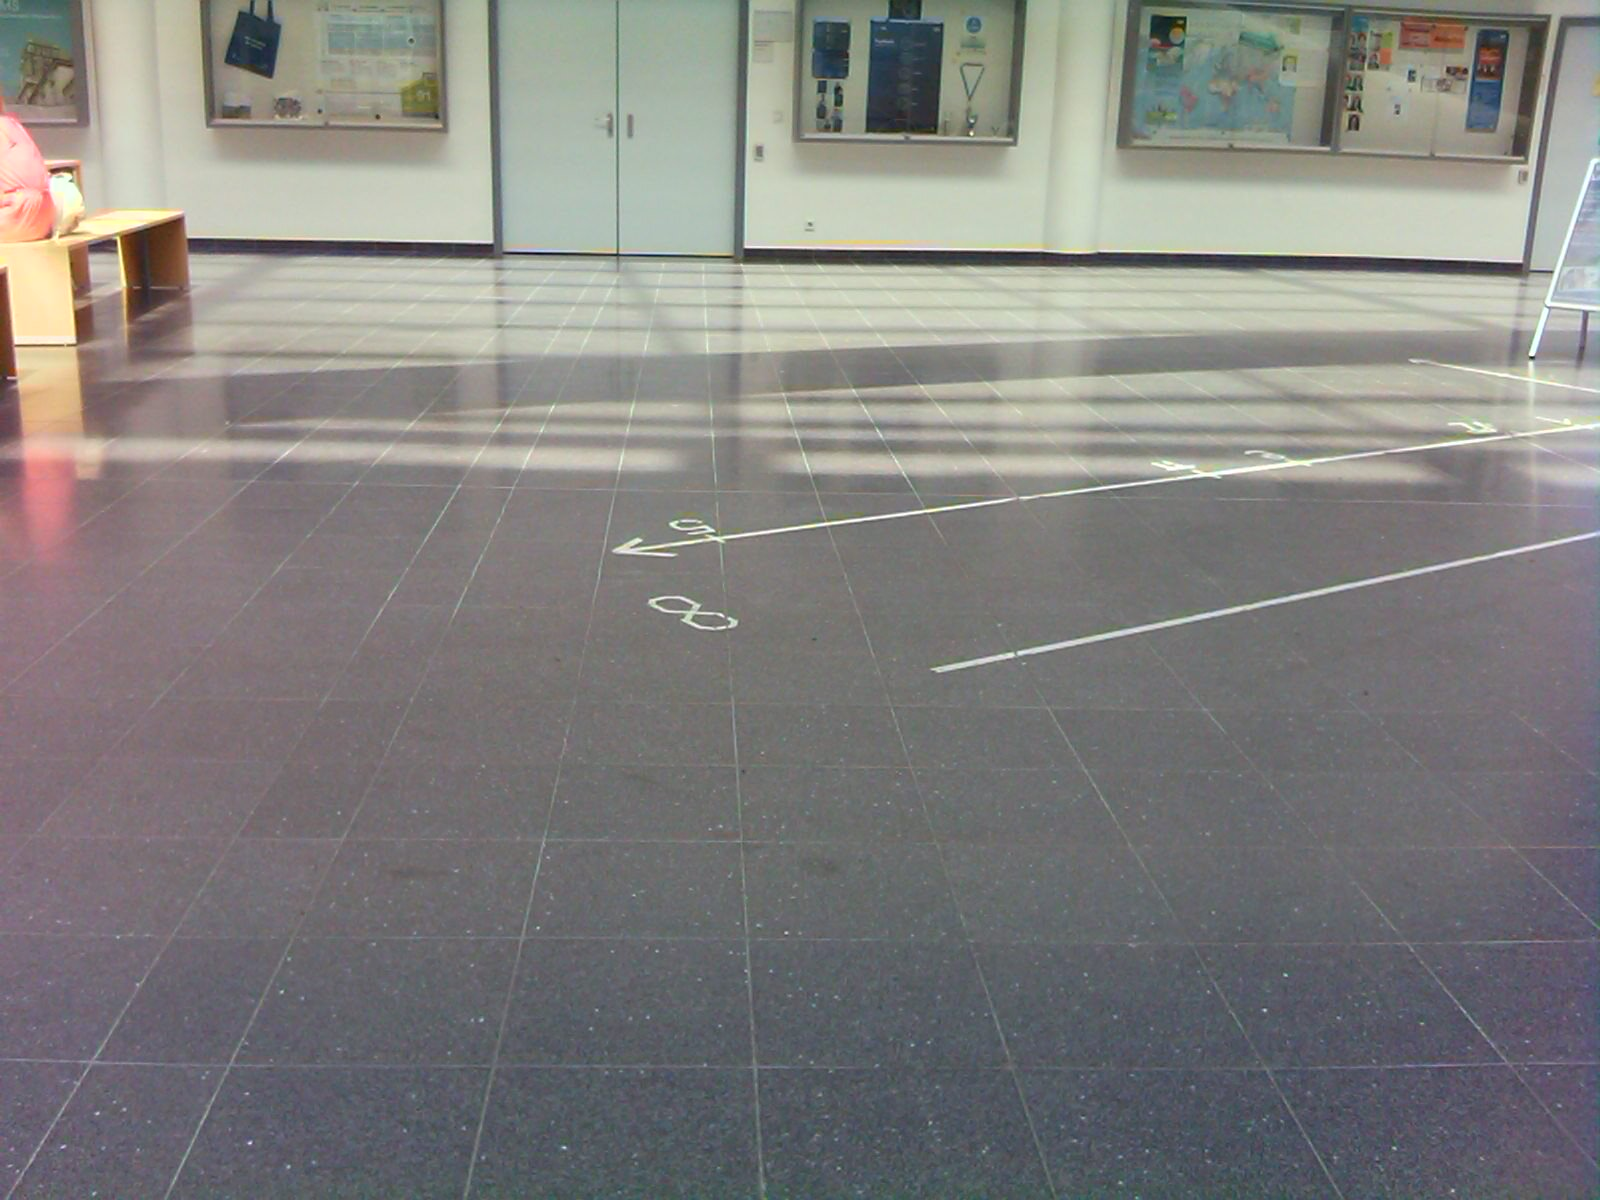
\includegraphics[scale=0.1]{tiles}
\end{figure}
Size of the main hall: on average 150m length, 19m width
\end{frame}

\begin{frame}{Complex geometry in the code}
 How to define the geometry, the flagfield for such a complex geometry?
 \begin{itemize}
  \item Use an external script to set the flagfield for every subdomain
  \item Set different flags for the different boundaries
 \end{itemize}

\end{frame}


\section{Challenges}
\begin{frame}{Challenges}
 \begin{itemize}
  \item How to separate such a complex geometry?
  \begin{itemize}
   \item Approach \#1: Focus on the specific scenario and specific values
   for number of processes
   \item Approach \#2: Divide the geometry to smaller blocks and assign multiple
   blocks to each processor (how to optimize communication?)
  \end{itemize}
 \item How to define the connections between the blocks?
 \item How to deal with the multiple boundary conditions?
 \pause
 \item Can we solve a fine-enough grid on our laptops?
 \end{itemize}

\end{frame}

\section*{Questions}
\begin{frame}{Thank you!}
 We are open for questions and ideas!
\end{frame}







\end{document}
